%%%%%%%%%%%%%%%%%%%%%%%%%%%%%%%%%%%%%%%%%
% Short Sectioned Assignment
% LaTeX Template
% Version 1.0 (5/5/12)
%
% This template has been downloaded from:
% http://www.LaTeXTemplates.com
%
% Original author:
% Frits Wenneker (http://www.howtotex.com)
%
% License:
% CC BY-NC-SA 3.0 (http://creativecommons.org/licenses/by-nc-sa/3.0/)
%
%%%%%%%%%%%%%%%%%%%%%%%%%%%%%%%%%%%%%%%%%

%----------------------------------------------------------------------------------------
%   PACKAGES AND OTHER DOCUMENT CONFIGURATIONS
%----------------------------------------------------------------------------------------

\documentclass[paper=a4, fontsize=11pt]{scrartcl} % A4 paper and 11pt font size


\usepackage[polish]{babel}
\usepackage[utf8]{inputenc}
\usepackage[T1]{fontenc}
\DeclareUnicodeCharacter{00A0}{ }
\DeclareUnicodeCharacter{00A0}{~}
\usepackage{lmodern}
\selectlanguage{polish}
\usepackage{amsmath,amsfonts,amsthm} % Math packages
\usepackage{enumerate}
\usepackage{graphicx}
\DeclareGraphicsExtensions{.pdf,.png,.jpg}
\usepackage{enumitem}
\setlength\parindent{0pt} % Removes all indentation from paragraphs - comment this line for an assignment with lots of text
\usepackage{tabularx}

%----------------------------------------------------------------------------------------
%   TITLE SECTION
%----------------------------------------------------------------------------------------

\newcommand{\horrule}[1]{\rule{\linewidth}{#1}} % Create horizontal rule command with 1 argument of height

\title{ 
    \normalfont \normalsize 
    \textsc{Politechnika Warszawska} \\ [25pt] % Your university, school and/or department name(s)
    \horrule{0.5pt} \\[0.4cm] % Thin top horizontal rule
    \huge Specyfikacja techniczna systemu informatycznego firmy Park-ex\\ % The assignment title
    \horrule{2pt} \\[0.5cm] % Thick bottom horizontal rule
}

\author{Mateusz Starzycki} % Your name

\date{\normalsize\today} % Today's date or a custom date

\begin{document}

\maketitle % Print the title

\newpage

\tableofcontents

%----------------------------------------------------------------------------------------
%   PROBLEM 1
%----------------------------------------------------------------------------------------

\newpage
\section{Wstęp }

Przedstawicielstwo firmy park-ex zdecydował się na renowacje systemu zarządzania firmą.
W tym celu zgłosił się do naszej firmy konsultingowej w celu zlecenia wykonania systemu informatycznego.
Ninijeszy dokument jest zbiorem wymagań zebranych podczas wywiadu z klientem przez analityków naszej firmyz

\section{Wizja system}

System informatyczny ma za zadanie pomoc w administracji parkingami firmy park-ex. Przedstawicielstwo firmy jest zainteresowane 
wprowadzeniem systemu informatyzcnego głownie z powodu na problem zarządzania firmą. Technologia obecnie używana jest
przestarzała - firma używa papierowych dokumentów których organizacja pochłania środki i czas. 

Główne korzyści dla firmy to możliwość zmniejszenia ilości czasu na żmudne procesy administracji oparte o dokumenty papierowe. Zmniejszenie
kosztów przechowywania i administracji, oraz możliwość uruchomienia dodatkowych programów dla klientów.

System ma zatem umożliwić przyspieszoną administrację firmą. W skład administracji wchodzi zarządzanie płatnościami oraz rezerwacjami a także
pomoc w codziennej pracy administratorów i nadzorców parkingów.

\subsection{Cechy systemu}

Cechy zostały zgrupowane w kategorii w zależności od użytkownika systemu.
Zidentyfikowanychzostało pięć kategorii systemu:

\begin{itemize}
  \item Użytkownik parkingu
  \item Pracownik nadzoru parkingu
  \item Pracownik administracji
  \item Manager firmy
  \item Administrator systemu 
\end{itemize}

W zależności od przynależności potrzeby użytkownika są różne, a także ciężar położony jest na inne aspekty.
Niniejszy rozdział skupia się na zidentyfikowaniu najważniejszych aspektów systemu.
Ogólne wymagania stawiane systemowi to dość duża niezawodność, możliwość prowadzenia pracy na parkingu
w przypadku awarii internetu, oraz bezpieczeństwo danych firmy.

\subsubsection{Użytkownik parkingu}

Najważniejszym aspektem użytkownika zewnętrznego jest dostępność oraz przejżystość informacji na stronie firmy.
Niesie to ze sobą potrzebę zalogowania się oraz ograniczenia dostępu zewnętrznego użytkownika do systemu.
Użytkownik zewnętrzny musi mieć dostęp do historii płatności za parking, możliwość opłacenia kolejnych miesiąców.
Dla użytkowników nie objętych kontraktem niezbędna jest informacja on-line o stanie parkingu.
Muszą oni także mieć możliwość rezerwacji krótkoterminowej parkingu.
Dodatkowo ma on także możliwość modyfikacji swoich danych osobowych.

Do rejestracji stałych klientów niezbędne są karty magnetyczne, co za tym idzie użytkownik może poprzez interfejs zgłosić potrzebę wydania nowej, oraz zgłoszenia
zepsucia lub zgubienia starej karty. Użytkownik może także zrezygnować z usług firmy przez stronę internetową.
Dodatkowo możliwe jest też zgłoszenie długotrwałego wyjazdu, co pozwoli parkingowi na ponowne wynajęcie miejsca parkingowego,
a użytkownikowi pozwoli zmniejszyć koszty płacone za miejsce parkingowe podczas jego nieobecnośći.

Podsumowując wymagania użytkownika parkingu można przedstawić następująco:

\begin{enumerate}
  \item Użytkownik zakłada konto w systemie
  \item Użytkownik loguje się do systemu
  \item Użytkownik przegląda historię płatności
  \item Użytkownik dokonuje rezerwacji postoju krótkoterminowego
  \item Użytkownik dokonuje rezerwacji postoju długoterminowego
  \item Użytkownik dokonuje płatności
  \item Użytkownik zgłasza prośbę wydania nowej karty
  \item Użytkownik zgłasza zaginioną kartę
  \item Użytkownik zgłasza wyjazd długoterminowy
\end{enumerate}


\subsubsection{Pracownik nadzoru parkingu}

Pracownik nadzoru parkingu przykłada największą wagę do łatwości oraz niezawodności interfejsu parkowania.
W celu ułatwienia zarządzania parkingiem musi on mieć informacje na temat stanu abonamentu nadjeżdzających klientów.
Dodatkowym wymaganiem administracyjnym jest także ustawienie nocnych powiadomień obchodowych - pracownik musi co jakiś czas
obejść parking oraz zalogować ten fakt w systemie. Dodatkowym wymaganiem systemu jest także automatyczne logowanie przyjeżdzających
oraz wyjeżdżających klientów z parkingu. System musi także być niezawodny - w wyniku natury pracy dostęp do internetu nie jest zawsze
gwarantowany - musi istnieć możliwość pracy w trybie bez połączenia z internetem i późniejsza synchronizacja.
Ostatnim wymogiem systemu jest możliwość alarmowego wezwania brygady ochrony, w przypadku zaistnienia incydentu, pracownik
nadzoru musi zawiadomić firmę ochronną w celu interwencji.

\begin{enumerate}
  \item Pracownik loguje się do sytemu
  \item Pracownik przegląda informacje nadjeżdzającego klienta
  \item Pracownik przegląda rezerwacje krótkoterminowe
  \item Pracownik zgłasza alarm w przypadku incydentu
  \item Pracownik zostaje przypomniany o nadchodzącej godzinieobchodu nocnego
\end{enumerate}

\subsubsection{Pracownik administracji}

Pracownik administracji w firmie zajmuje się głównie kontaktami z klientem oraz administracją konta klientów.
System informatyczny ma być dla niego ułatwieniem polegającym na automatycznym wyszukiwaniu klientów o wygasających kontraktach.
Dodatkowo pracownik administracji musi mieć dostęp do danych płatności oraz raportów płatności w celu ułatwienia księgowania
oraz raportowania zysków.

\begin{enumerate}
  \item Pracownik wyświetla dane klientów o konczących się terminach umowy 
  \item Pracownik wyświetla dane osobowe klientów w celu wysłania kart parkingowych
  \item Pracownik generuje raport
\end{enumerate}

\subsubsection{Manager firmy}

Manager firmy będzie używać systemu jako narzędzia wspomagającego decyzje o przyszłości firmy. Ma on mieć możliwość 
wglądu w zyski z poszczególnych siedzib, dane o ilości klientów, ich wzroście, dostęp do historii cen miejsc parkingowych
w poszczególnych gałęziach firmy.

\begin{enumerate}
  \item Manager generuje raport
  \item Manager przegląda historyczne raporty
\end{enumerate}

\subsubsection{Administrator systemu }

Główną rolą administratora jest tworzenie kont pracowniczych, dodawanie nowych gałęźi firmy do systemu.
Administrator musi także posiadać informacje dotyczące łączności poszczególnych parkingów do centrali.
Dodatkowo musi on także posiadać możliwość tworzenia automatycznego, oraz ręcznego back upów systemu.
Ostatnim wymaganiem jest możliwość przywracania systemu do stanu zapisanego w back-upie. Proces ten musi 
zostać zatwierdzony przez managera firmy. Administrator nie powinien mieć dostępu do danych finansowych firmy,
oraz danych osobowych jej klientów.


\begin{enumerate}
  \item Administrator dodaje użytkownika do systemu
  \item Administrator wykonuje kopie zapasowa systemu
  \item Administrator przywraca kopie systemu
\end{enumerate}

\section{Wymagania użytkownika}

\subsection{Wymagania funkcjonalne}

Sekcja ta opisuje wymagania funkcjonalne stawiane systemowi. 
Zostały one podzielone na pare kategorii, ze względu na różne obszary zastosowań systemu.

\subsubsection{Stały Klient Firmy Park-Ex}

\begin{itemize}
\item Zakładanie konta w systemie
\item Logowanie do systemu
\item Przeglądanie historii płatności
\item Przeglądanie danych osobowych
\item Edycja danych profilu
\item Zgłaszanie długoterminowego wyjazdu
\item Zamówienie nowej karty
\item Zgłoszenie ukradzionej / zaginionej karty
\end{itemize}

\subsubsection{Klient jednorazowy}

\begin{itemize}
\item Sprawdzenie dostępności miejsc parkingowych
\item Rezerwacja miejsc parkingowych z płatnością
\end{itemize}


Diagram scenariuszy użycia klienta:

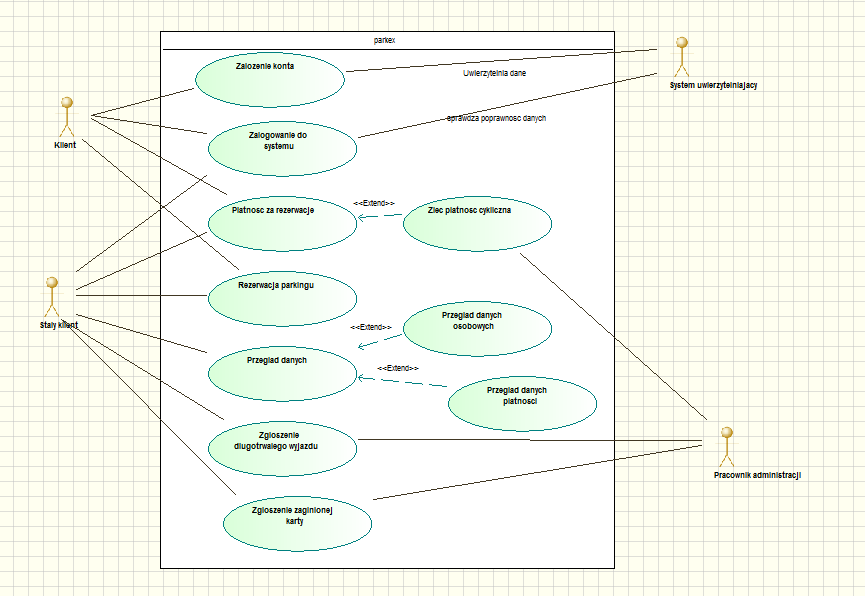
\includegraphics[scale=0.7]{kli}

\subsubsection{Pracownik nadzoru parkingu}

\begin{itemize}
\item Wyświetlenie profilu nadjeżdżającego klienta
\item Wyszukanie tymczasowego klienta w systemie
\item Przycisk alarmowy
\item Przypomnienie o obchodzie nocnym
\end{itemize}


Diagram przypadków użycia:

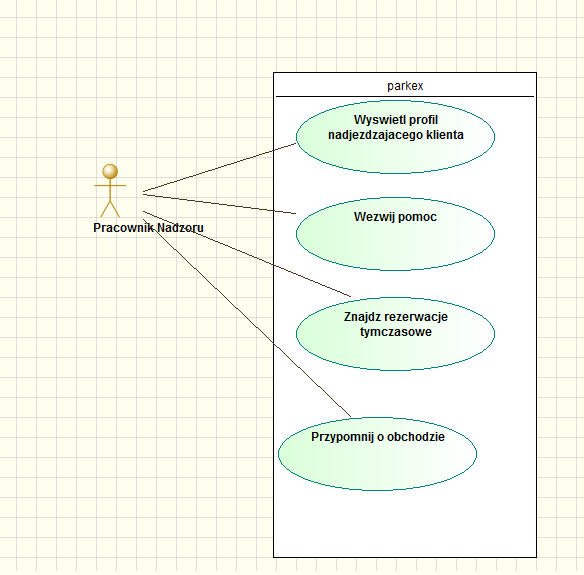
\includegraphics[scale=0.7]{pnad}

\subsubsection{Pracownik Administracji}

\begin{itemize}
\item Wyświetlenie profili użytkowników o nadchodzącym terminie końca umowy
\item Wyświetlenie danych płatności klientów oraz wyszukiwanie klientów w bazie danych
\item Wyświetlenie wniosków wydania nowych kart oraz danych osobowych klientów
\end{itemize}

Diagram przypadków użycia:

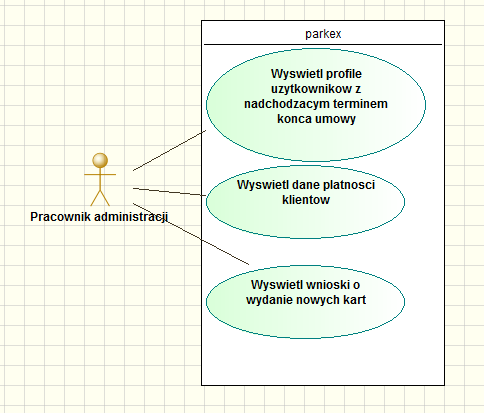
\includegraphics[scale=0.7]{padm}

\subsubsection{Manager Firmy}

\begin{itemize}
\item Generacja raportów użytkowania parkingów
\item Raporty zarobków w różnych filiach firmy.
\end{itemize}

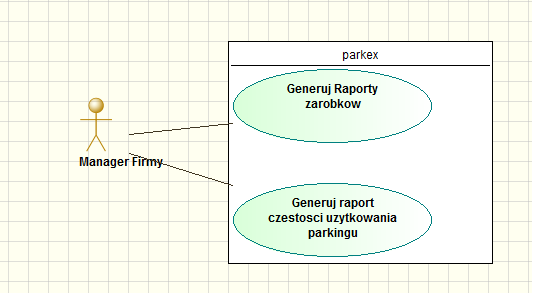
\includegraphics[scale=0.7]{mana}

\subsubsection{Administrator Systemu}

\begin{itemize}
\item Wyświetlenie statusu połączeń parkingów
\item Dodanie użytkownika do systemu
\item Dodatnie siedziby do systemu
\item Back-up systemu
\item Przywrócenie stanu z przed back upu systemu.
\end{itemize}

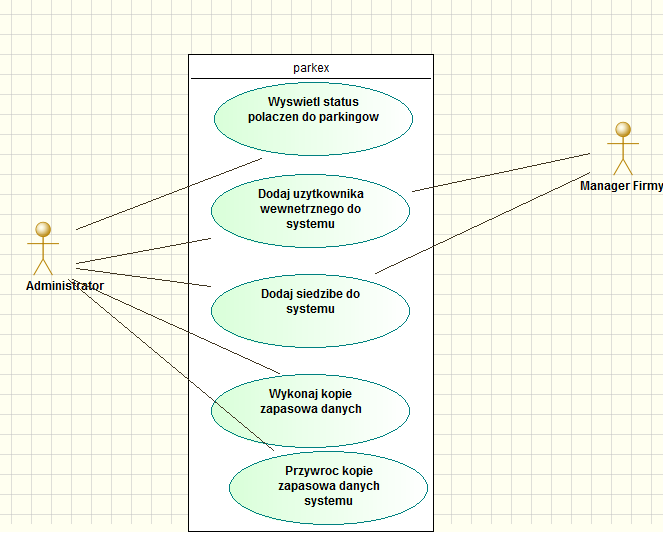
\includegraphics[scale=0.7]{admin}

\subsection{Wymagania jakościowe}

\subsubsection{Funkcjonalność}

\begin{tabularx}{\textwidth}{|r|X|}
  \hline
Treść wymagania  & System będzie umożliwiał wykorzystanie wszystkich scenariuszy przypadków użycia. \\ 
  \hline
Sposób testowania  & Testy akceptacyjne użytkownika. \\ 
  \hline
Matryka pomiaru  & Test dotyczący każdego scenariusza - użytkownik będzie przechodził przez poszczególne scenariusze i zatwierdzać będzie pomyślne przejście przez przypadek użycia. \\ 
  \hline
\end{tabularx}

\vspace{10 mm}

\begin{tabularx}{\textwidth}{|r|X|}
  \hline
Treść wymagania  & System będzie prosty i intuicyjny w obsłudze. \\ 
  \hline
Sposób testowania  & Testy zdolności użytkownika do nauczenia się w tydzień interfejsów programu. \\ 
  \hline
Metryka pomiaru  & Po tygodniowym szkoleniu zostaną poddani pracownicy firmy oraz losowe gronoosób w roli użytkownika zewnętrznego, wynikiem przejścia testu będzie przejście 80\% użytkowników. \\ 
  \hline
\end{tabularx}

\vspace{10 mm}

\begin{tabularx}{\textwidth}{|r|X|}
  \hline
Treść wymagania  & Zadowolenie użytkownika. \\ 
  \hline
Sposób testowania  & Ankieta po okresie próbnym użytkowania systemu, dotycząca łatwości obsługi, dostępności funkcji, intuicyjności oraz szybkości obsługi systemu. \\ 
  \hline
Metryka pomiaru  & Procent zadowolonych użytkowników musi wynosić więcej niz 80\%. \\ 
  \hline
\end{tabularx}

\subsubsection{Niezawodność}

\begin{tabularx}{\textwidth}{|r|X|}
  \hline
Treść wymagania & System będzie w stanie działać w przypadku zerwania łączności z internetem. \\ 
  \hline
Sposób testowania & Odłączenie komputera z systemem od sieci. \\ 
  \hline
Metryka pomiaru & System utrzyma stabilność w przypadku 95\% odłączeń od sieci. Dodatkowym parametrem
akceptacyjnym będzie także czas synchronizacji systemu po podłączeniu do sieci który zawsze ma wynosić mniej niz
30 sekund. \\ 
  \hline
\end{tabularx}

\vspace{10 mm}

\begin{tabularx}{\textwidth}{|r|X|}
  \hline
Treść wymagania & System będzie działać stabilnie po wdrożeniu do środowiska klienta. \\ 
  \hline
Sposób testowania & Testowanie poprzez wdrożenie wstępne oraz zbieranie logów z błędów systemu. \\ 
  \hline
Metryka pomiaru & System ma dla każdego użytkownika zawierać conajwyżej 1 błąd krytyczny w ciągu miesiąca
działalności programu oraz maksymalnie 4 błedy nie krytyczne. \\ 
  \hline
\end{tabularx}

\subsubsection{Wydajność}

\begin{tabularx}{\textwidth}{|r|X|}
  \hline
Treść wymagania & Małe zużycie pamięci RAM \\ 
  \hline
Sposób testowania & Skrypt działający w tle systemu operacyjnego mający wgląd w zużycie pamięci przez poszczególne procesy. \\ 
  \hline
Metryka pomiaru & Procent zużytej pamięci - wartość nie może przekraczać 50\%. \\ 
  \hline
\end{tabularx}

\vspace{10 mm}

\begin{tabularx}{\textwidth}{|r|X|}
  \hline
Treść wymagania & Szybka możliwość back upu danych. \\ 
  \hline
Sposób testowania & Skrypt mierzący czas pomiędzy rozpoczęciem zrzutu bazy danych systemu a jego końcem. \\ 
  \hline
Metryka pomiaru & Back up ma być wykonany szybciej niż 20 minut. \\ 
  \hline
\end{tabularx}

\vspace{10 mm}

\begin{tabularx}{\textwidth}{|r|X|}
  \hline
Treść wymagania & Możliwość szybkiej synchronizacji po utraceniu łaczności z internetem. \\ 
  \hline
Sposób testowania & Skrypt mierzący czas pomiędzy podłączeniem internetu a wiadomością pełnej synchronizacji. \\ 
  \hline
Metryka pomiaru & Czas musi być krótszy niż 30 sekund. \\ 
  \hline
\end{tabularx}

\subsubsection{Łatwość utrzymania}

\begin{tabularx}{\textwidth}{|r|X|}
  \hline
Treść wymagania & Dobra dokumentacja techniczna\\ 
  \hline
Metryka pomiaru & Akceptacja klienta\\ 
  \hline
\end{tabularx}

\vspace{10 mm}

\begin{tabularx}{\textwidth}{|r|X|}
  \hline
Treść wymagania & Dostępność oraz przejrzystość dokumentacji użytkowej\\ 
  \hline
Sposób testowania & Akceptacja klienta\\ 
  \hline
Metryka pomiaru & Dokumentacja musi zostać zaakceptowana przez klienta.\\ 
  \hline
\end{tabularx}

\subsubsection{Przenośność}

Brak potrzeby testowania przenośności - klient chce użytkować systemu na znanym hardwarze.

\subsection{Słownik użytkownika}

Rozdział ten poświęcony jest definicji aktorów oraz elementów systemu 

\subsubsection{Aktorzy systemu}

Aktorami systemu są:

\begin{itemize}
  \item Użytkownik parkingu
  \item Pracownik nadzoru parkingu
  \item Pracownik administracji
  \item Manager firmy
  \item Administrator systemu 
\end{itemize}

\subsubsection{Pojęcia dziedziny}

Poniższy diagram predstawia mapę pojęć dziedziny:

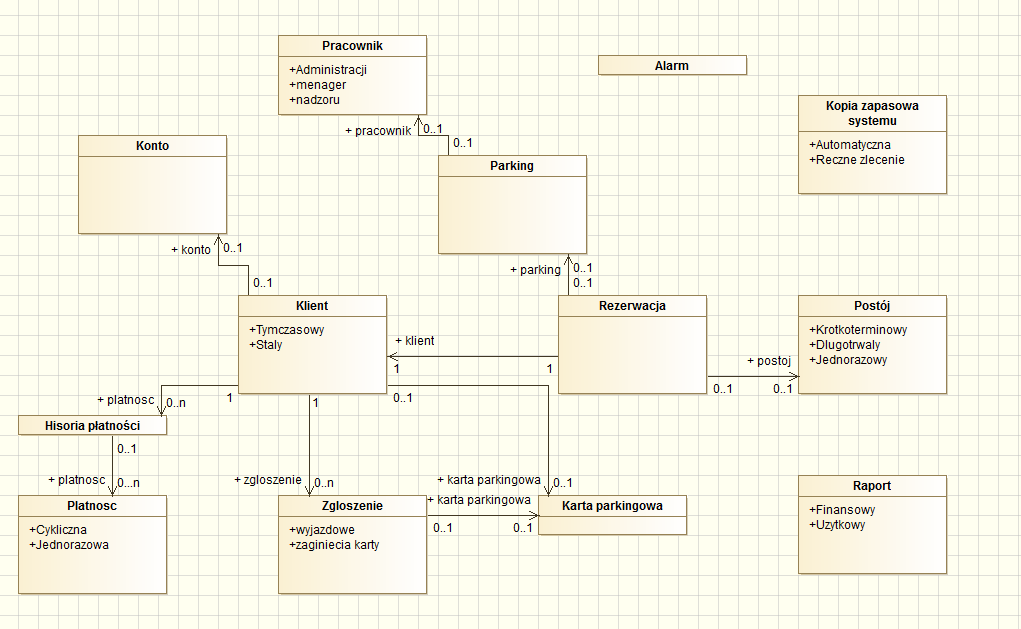
\includegraphics[scale=0.5]{slownik}

Opis pojęć dziedziny:


\begin{description}
  \item[Raport] Dokument przedstawiający zbiór danych firmy na przestrzeni czasu.
  \item[Raport Finansowy] Dokument przedstawiający dane przychodów firmy w danych jej filiach w wybranej przestrzeni czasu
  \item[Pracownik Administracji] Osoba zajmująca się zarządzaniem kontami klientów firmy oraz utrzymująca z nimi kontakty.
  \item[Pracownik Nadzoru] Osoba zatrudniona na stanowisku ochroniarza w filii firmy.
  \item[Administrator] Osoba zajmująca się systemem informatycznym firmy Park-ex.
  \item[Dane Osobowe] Wszelkie dane klienta które umożliwiają jego identyfikację.
  \item[Dane Finansowe] Wszelkie informacje dotyczące przychodów lub rozchodów firmy.
  \item[Platność cykliczna] Ustalony comiesięczny przelew za usługi świadczone przez firmę Park-ex.
  \item[Płatność jednorazowa] Płatność za jeden miesiąc parkingu lub pojedyńczą rezerwację.
  \item[Zgłoszenie wyjazdowe] Usługa polegająca na zgłoszeniu dłuższej nieobecności stałego klienta, umożliwia ona obniżenie kosztów klienta.
  \item[Klient Tymczasowy] Klient rezerwujący jednorazowy pobyt na parkingu Park-ex.
  \item[Klient Stały] Klient posiadający konto w systemie.
  \item[Rezerwacja] Zgłoszona w systemie chęc skorzystania z usłóg firmy Park-ex.
  \item[Postój jednorazowy] Postój trwający mniej niż jeden dzien.
  \item[Postój krótkotrwały]Postój trwający mniej niż jeden miesiąc.
  \item[Postój długotrwały] Postój trwający więcej niż jeden miesiąc.
  \item[Karta Parkingowa] Identyfikator - karta umożliwiająca identyfikację klienta. Niezbędna dla klientów stałych o usługach długoterminowych.
\end{description}

\paragraph{Elementy interfejsu użytkownika}

Interfejs użytkownika będzie oparty o stronę www.
Zostanie ona utworzona z użyciem technologii bootstrap.


Zaprezentowane też zostaną w tym rozdziale dwa najciekawsze scenariusze użytkowania systemu.

Dodawanie cyklicznego tworzenia kopii zapasowej:

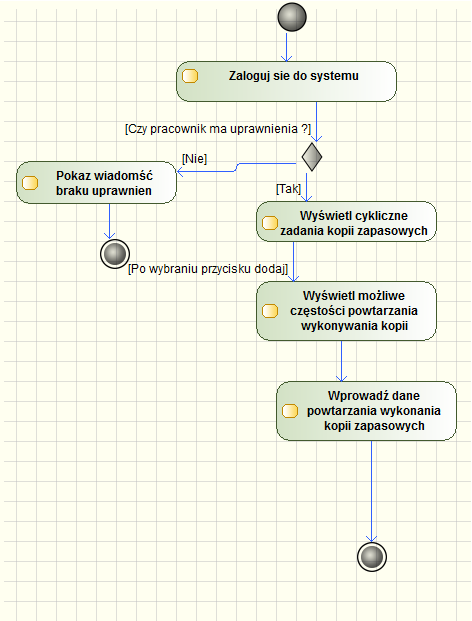
\includegraphics[scale=0.7]{1}

Dokonywania rezerwacji w systemie:

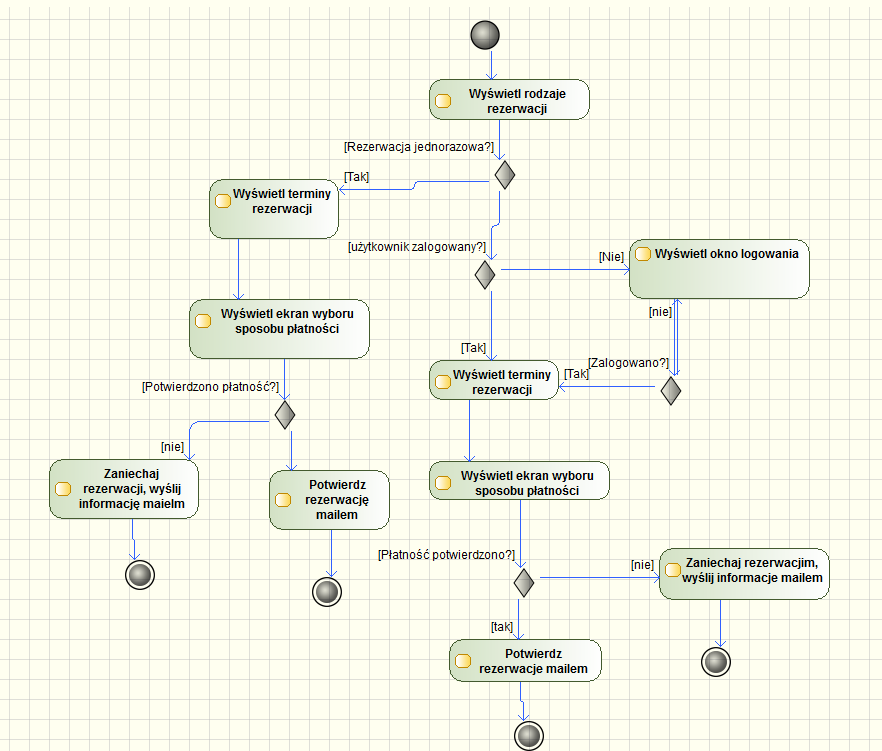
\includegraphics[scale=0.7]{2}

Zgłaszania wyjazdu długoterminowego:

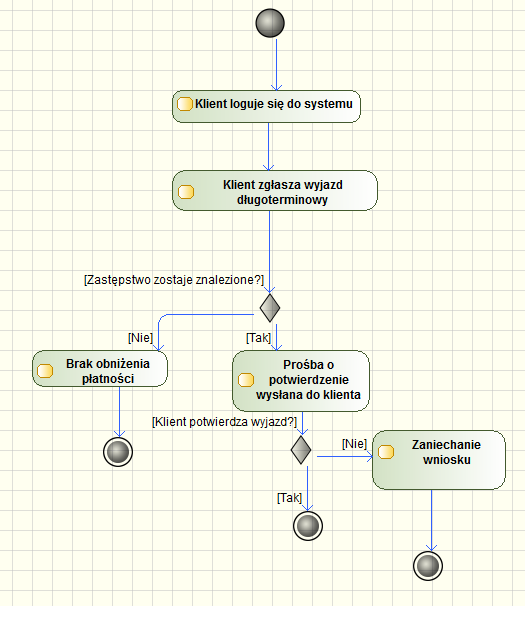
\includegraphics[scale=0.7]{3}

Proces rejestracji jako stały klient firmy Park-ex:

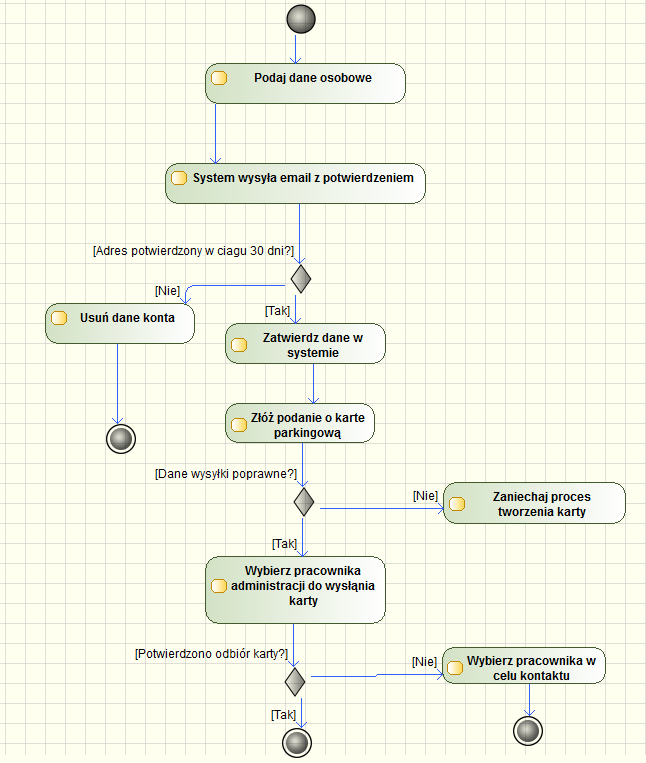
\includegraphics[scale=0.7]{4}

\paragraph{Elementy i parametry systemu}

\begin{itemize}
  \item Ilość parkowanych samochodów
  \item Ilość kont użytkowników
  \item Ilość filii firmy
  \item Ilość pracowników firmy
  \item Ilość rezerwacji
  \item Ilość serwerów
  \item Średni czas dostępu klienta 
  \item Ilość danych w bazie danych
\end{itemize}

\end{document}
